\documentclass[11pt]{article}

\usepackage{blindtext}
\usepackage{graphicx}

\title{Plato's Life}

\author{Tejas Sanap}

\date{\today}

\begin{document}
	\maketitle

	\section{Introduction}
		% fix quotes and ---
		% Plato (429?–347 B.C.E.) is, by any reckoning, one of the most dazzling writers in the Western literary tradition and one of the most penetrating, wide-ranging, and influential authors in the history of philosophy. An Athenian citizen of high status, he displays in his works his absorption in the political events and intellectual movements of his time, but the questions he raises are so profound and the strategies he uses for tackling them so richly suggestive and provocative that educated readers of nearly every period have in some way been influenced by him, and in practically every age there have been philosophers who count themselves Platonists in some important respects. He was not the first thinker or writer to whom the word “philosopher” should be applied. But he was so self-conscious about how philosophy should be conceived, and what its scope and ambitions properly are, and he so transformed the intellectual currents with which he grappled, that the subject of philosophy, as it is often conceived—a rigorous and systematic examination of ethical, political, metaphysical, and epistemological issues, armed with a distinctive method—can be called his invention. Few other authors in the history of Western philosophy approximate him in depth and range: perhaps only Aristotle (who studied with him), Aquinas, and Kant would be generally agreed to be of the same rank.

		Plato (429?–347 B.C.E.) is, by any reckoning, one of the most dazzling writers in the Western literary tradition and one of the most penetrating, wide-ranging, and influential authors in the history of philosophy. An Athenian citizen of high status, he displays in his works his absorption in the political events and intellectual movements of his time, but the questions he raises are so profound and the strategies he uses for tackling them so richly suggestive and provocative that educated readers of nearly every period have in some way been influenced by him, and in practically every age there have been philosophers who count themselves Platonists in some important respects. He was not the first thinker or writer to whom the word ``philosopher" should be applied. But he was so self-conscious about how philosophy should be conceived, and what its scope and ambitions properly are, and he so transformed the intellectual currents with which he grappled, that the subject of philosophy, as it is often conceived --- a rigorous and systematic examination of ethical, political, metaphysical, and epistemological issues, armed with a distinctive method --- can be called his invention. Few other authors in the history of Western philosophy approximate him in depth and range: perhaps only Aristotle (who studied with him), Aquinas, and Kant would be generally agreed to be of the same rank.

	\section{Who is Plato?}
		% fix image size and add caption and stuff

		% 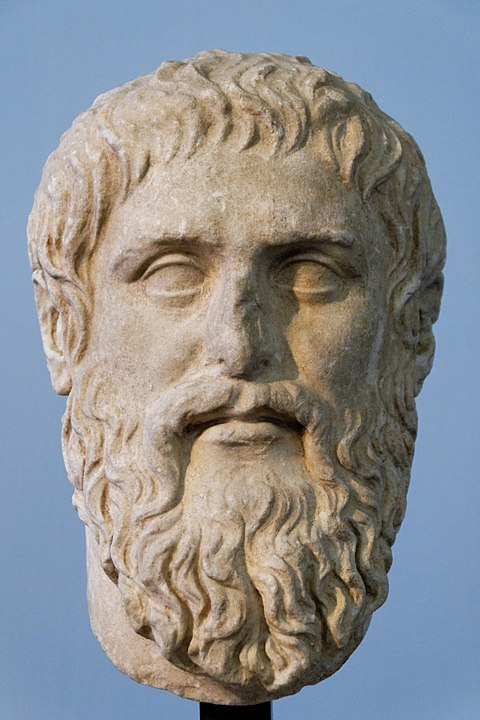
\includegraphics{images/plato_bust.jpg}

		% 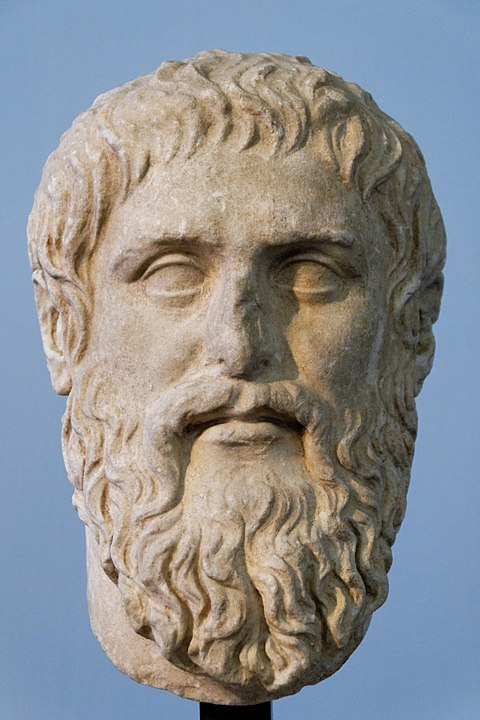
\includegraphics[width=0.3\textwidth, keepaspectratio]{images/plato_bust.jpg}

		% \begin{figure}[h]
		% 	\centering
		% 	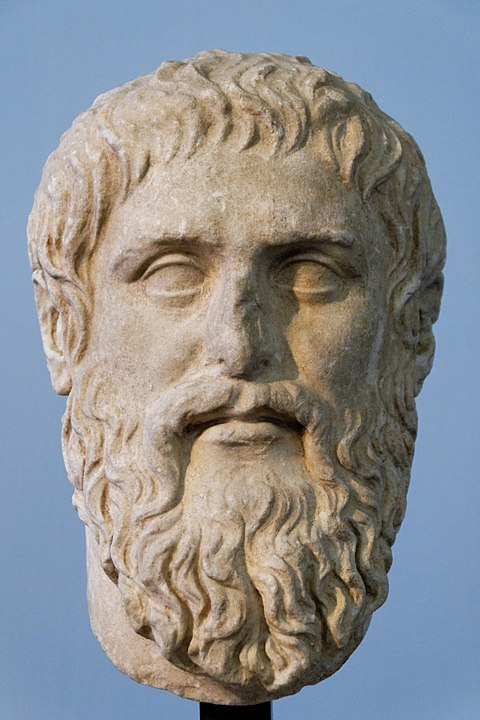
\includegraphics[width=0.3\textwidth, keepaspectratio]{images/plato_bust.jpg}
		% 	\caption{Plato's potrait bust}
		% 	\label{img:platobust}
		% \end{figure}

		% remove wiki references - search and replace - \[\d*\]

		%The specific birthdate of Plato is not known. Based on ancient sources, most modern scholars estimate that Plato was born between 428 and 427 BC. The grammarian Apollodorus of Athens argues in his Chronicles that Plato was born in the first year of the eighty-eighth Olympiad (427 BC), on the seventh day of the month Thargelion; according to this tradition the god Apollo was born this day.[2] According to another biographer of him, Neanthes, Plato was eighty-four years of age at his death.[3] If we accept Neanthes' version, Plato was younger than Isocrates by six years, and therefore he was born in the second year of the 87th Olympiad, the year Pericles died (429 BC).[4]
		%The Chronicle of Eusebius names the fourth year of the 89th Olympiad as Plato's, when Stratocles was archon, while the Alexandrian Chronicle mentions the eighty-ninth Olympiad, in the archonship of Isarchus.[5] According to Suda, Plato was born in Aegina in the 88th Olympiad amid the preliminaries of the Peloponnesian war, and he lived 82 years.[6] Sir Thomas Browne also believes that Plato was born in the 88th Olympiad.[7] Renaissance Platonists celebrated Plato's birth on November 7.[8] Ulrich von Wilamowitz-Moellendorff estimates that Plato was born when Diotimos was archon eponymous, namely between July 29 428 BC and July 24 427 BC.[9] Greek philologist Ioannis Kalitsounakis believes that the philosopher was born on May 26 or 27, 427 BC, while Jonathan Barnes regards 428 BC as year of Plato's birth.[10] For her part, Debra Nails asserts that the philosopher was born in 424/423 BC.[8]
		%Plato's birthplace is also disputed. Diogenes Laërtius states that Plato "was born, according to some writers, in Aegina in the house of Phidiades the son of Thales". Diogenes mentions as one of his sources the Universal History of Favorinus. According to Favorinus, Ariston and his family were sent by Athens to settle as cleruchs (colonists retaining their Athenian citizenship), on the island of Aegina, from which they were expelled by the Spartans after Plato's birth there.[3] Nails points out, however, that there is no record of any Spartan expulsion of Athenians from Aegina between 431 and 411 BC.[11] On the other hand, at the Peace of Nicias, Aegina was silently left un der Athens control, and it was not until the summer of 411 that the Spartans overran the island.[12] Therefore, Nails concludes that "perhaps Ariston was a cleruch, perhaps he went to Aegina in 431, and perhaps Plato was born on Aegina, but none of this enables a precise dating of Ariston's death (or Plato's birth)".[11] Aegina is regarded as Plato's place of birth by Suda as well.[6]

		The specific birthdate of Plato is not known. Based on ancient sources, most modern scholars estimate that Plato was born between 428 and 427 BC. The grammarian Apollodorus of Athens argues in his Chronicles that Plato was born in the first year of the eighty-eighth Olympiad (427 BC), on the seventh day of the month Thargelion; according to this tradition the god Apollo was born this day. According to another biographer of him, Neanthes, Plato was eighty-four years of age at his death. If we accept Neanthes' version, Plato was younger than Isocrates by six years, and therefore he was born in the second year of the 87th Olympiad, the year Pericles died (429 BC).

		The Chronicle of Eusebius names the fourth year of the 89th Olympiad as Plato's, when Stratocles was archon, while the Alexandrian Chronicle mentions the eighty-ninth Olympiad, in the archonship of Isarchus. According to Suda, Plato was born in Aegina in the 88th Olympiad amid the preliminaries of the Peloponnesian war, and he lived 82 years. Sir Thomas Browne also believes that Plato was born in the 88th Olympiad. Renaissance Platonists celebrated Plato's birth on November 7. Ulrich von Wilamowitz-Moellendorff estimates that Plato was born when Diotimos was archon eponymous, namely between July 29 428 BC and July 24 427 BC. Greek philologist Ioannis Kalitsounakis believes that the philosopher was born on May 26 or 27, 427 BC, while Jonathan Barnes regards 428 BC as year of Plato's birth. For her part, Debra Nails asserts that the philosopher was born in 424/423 BC.

		Plato's birthplace is also disputed. Diogenes Laërtius states that Plato ``was born, according to some writers, in Aegina in the house of Phidiades the son of Thales". Diogenes mentions as one of his sources the Universal History of Favorinus. According to Favorinus, Ariston and his family were sent by Athens to settle as cleruchs (colonists retaining their Athenian citizenship), on the island of Aegina, from which they were expelled by the Spartans after Plato's birth there. Nails points out, however, that there is no record of any Spartan expulsion of Athenians from Aegina between 431 and 411 BC. On the other hand, at the Peace of Nicias, Aegina was silently left under Athens control, and it was not until the summer of 411 that the Spartans overran the island. Therefore, Nails concludes that ``perhaps Ariston was a cleruch, perhaps he went to Aegina in 431, and perhaps Plato was born on Aegina, but none of this enables a precise dating of Ariston's death (or Plato's birth)". Aegina is regarded as Plato's place of birth by Suda as well.

\end{document}
